\section{Theoretical background}
\label{sec:pureshift__intro_theory}

In \cref{chpt:theory}, I showed how density operators could be expressed in either of the two bases $\{E, I_x, I_y, I_z\}$ or $\{E, I_z, I_+, I_-\}$, depending on which was most mathematically expedient.
To analyse pure shift NMR, it turns out to be most convenient to introduce a third basis, namely $\{I_\alpha, I_\beta, I_+, I_-\}$\autocite{Keeler2010,Thrippleton2005JMR,Griesinger1986JCP}.
The definitions of these terms are given in \cref{eq:other_single_spin_ops}: it is clear from there that, when expressed in the Zeeman basis, each matrix element of the density operator corresponds to one of these terms:
\begin{equation}
    \label{eq:single_element_operators}
    \rho = \begin{pmatrix}\rho_\alpha & \rho_+ \\ \rho_- & \rho_\beta\end{pmatrix}
     = \rho_\alpha I_\alpha + \rho_+ I_+ + \rho_- I_- + \rho_\beta I_\beta.
\end{equation}
In systems containing multiple spins, the corresponding \textit{single-element operators} are just the products of these operators.
In this section, I use a system with two weakly coupled spins $I_1$ and $I_2$ to illustrate the ideas behind pure shift NMR.
We have that $H_{\text{free},I} = \Omega_1 I_{1z} + \Omega_2 I_{2z} + 2\pi JI_{1z}I_{2z}$, which is diagonal in the Zeeman basis:
\begin{equation}
    \label{eq:h_free_weak}
    H_\text{free} = \begin{pmatrix}
        \omega_{\alpha\alpha} & 0 & 0 & 0 \\
        0 & \omega_{\alpha\beta} & 0 & 0 \\
        0 & 0 & \omega_{\beta\alpha} & 0 \\
        0 & 0 & 0 & \omega_{\beta\beta} \\
    \end{pmatrix}.
\end{equation}
Here, $\omega_{\lambda\mu} = \braket{\lambda\mu|H_{\text{free},I}|\lambda\mu}$ ($\lambda, \mu \in \{\alpha, \beta\}$) represents the precession frequency of the state $\ket{\lambda\mu}$.
Given that $I_z\ket{\alpha} = (1/2)\ket{\alpha}$ and $I_z\ket{\beta} = -(1/2)\ket{\beta}$, these frequencies are relatively easy to work out:
\begin{equation}
    \label{eq:state_precessions}
    \begin{aligned}
        \omega_{\alpha\alpha} &= \frac{1}{2}(\Omega_1 + \Omega_2 + \pi J), &
        \omega_{\alpha\beta} &= \frac{1}{2}(\Omega_1 - \Omega_2 - \pi J), \\
        \omega_{\beta\alpha} &= \frac{1}{2}(-\Omega_1 + \Omega_2 - \pi J), &
        \omega_{\beta\beta} &= \frac{1}{2}(-\Omega_1 - \Omega_2 + \pi J).
    \end{aligned}
\end{equation}
The corresponding propagator $U(\tau) = \exp(-\mi H_{\text{free},I}\tau)$ is then just:
\begin{equation}
    \label{eq:u_free_weak}
    U(\tau) = \begin{pmatrix}
        \exp(-\mi\omega_{\alpha\alpha}\tau) & 0 & 0 & 0 \\
        0 & \exp(-\mi\omega_{\alpha\beta}\tau) & 0 & 0 \\
        0 & 0 & \exp(-\mi\omega_{\beta\alpha}\tau) & 0 \\
        0 & 0 & 0 & \exp(-\mi\omega_{\beta\beta}\tau) \\
    \end{pmatrix}.
\end{equation}
Consequently, the evolution of the single-element operators under $H_{\text{free},I}$ is extraordinarily simple to calculate in matrix form: for example, we have that
\begin{equation}
    \label{eq:single_elem_plusalpha_evolution}
    I_{1+}I_{2\alpha} = \begin{pmatrix}
        0 & 0 & 1 & 0 \\
        0 & 0 & 0 & 0 \\
        0 & 0 & 0 & 0 \\
        0 & 0 & 0 & 0 \\
    \end{pmatrix},
\end{equation}
so $U(\tau) I_{1+} I_{2\alpha} \adj{U}(\tau)$ is
\begin{equation}
    \label{eq:single_elem_plusalpha_evolution_2}
    \begin{pmatrix}
        0 & 0 & \exp(-\mi\omega_{\alpha\alpha}\tau)\exp(\mi\omega_{\beta\alpha}\tau) & 0 \\
        0 & 0 & 0 & 0 \\
        0 & 0 & 0 & 0 \\
        0 & 0 & 0 & 0 \\
    \end{pmatrix} = \exp[-\mi(\Omega_1 + \pi J)\tau] I_{1+}I_{2\alpha}.
\end{equation}
Essentially, under $H_{\text{free},I}$, all of these operators acquire phase factors which depend on the difference between two of the frequencies $\omega_{\lambda\mu}$.
I explicitly state the rules for the single-quantum operators on spin 1 here:%
\footnote{Note that \S{} 10.4.2 of Keeler's text\autocite{Keeler2010} has a sign error in these equations---the sign of the $\pi J$ evolution is flipped---though it proves to be inconsequential as the sign of $J$ cannot be observed.}
\begin{align}
    I_{1+}I_{2\alpha} &\longrightarrow \exp[-\mi(\Omega_1 + \pi J)\tau] I_{1+}I_{2\alpha} \label{eq:shift_basis_evolution_pa} \\
    I_{1+}I_{2\beta} &\longrightarrow \exp[-\mi(\Omega_1 - \pi J)\tau] I_{1+}I_{2\beta} \label{eq:shift_basis_evolution_pb} \\
    I_{1-}I_{2\alpha} &\longrightarrow \exp[\mi(\Omega_1 + \pi J)\tau] I_{1-}I_{2\alpha} \label{eq:shift_basis_evolution_ma} \\
    I_{1-}I_{2\beta} &\longrightarrow \exp[\mi(\Omega_1 - \pi J)\tau] I_{1-}I_{2\beta} \label{eq:shift_basis_evolution_mb}
\end{align}
The rules for the corresponding operators on spin 2 can be easily obtained by permutation of labels.
Notice that the evolution frequencies of the $-1$-quantum operators (\cref{eq:shift_basis_evolution_ma,eq:shift_basis_evolution_mb}) each correspond to one peak of the corresponding multiplet in an NMR spectrum: for example, $\Omega_1 + \pi J$ and $\Omega_1 - \pi J$ correspond to the two peaks of the spin-1 doublet.

Consider now a simple spin echo sequence: $90^\circ_{x}$--$\tau$--$180^\circ_{x}$--$\tau$--detection.
The initial excitation pulse acts on both spins 1 and 2, and thus generates a mixture of all eight possible single-quantum operators (the four above plus four more on spin 2).
For simplicity, we consider only the $I_{1+}I_{2\alpha}$ term.
This evolves in the first $\tau$ delay to give $\exp[-\mi(\Omega_1 + \pi J)\tau] I_{1+}I_{2\alpha}$.
The $180^\circ$ pulse \textit{flips} both spins 1 and 2, in that it causes the transitions $I_+ \leftrightarrow I_-$ and $I_\alpha \leftrightarrow I_\beta$; consequently, we have that
\begin{equation}
    \label{eq:spin_echo_1}
    \exp[-\mi(\Omega_1 + \pi J)\tau] I_{1+}I_{2\alpha} \longrightarrow \exp[-\mi(\Omega_1 + \pi J)\tau] I_{1-}I_{2\beta}.
\end{equation}
In the second delay, we get a second phase factor from the evolution of the $I_{1-}I_{2\beta}$ operator:
\begin{align}
    \label{eq:spin_echo_2}
    \exp[-\mi(\Omega_1 + \pi J)\tau] I_{1-}I_{2\beta} \longrightarrow
    &\exp[-\mi(\Omega_1 + \pi J)\tau] \exp[\mi(\Omega_1 - \pi J)\tau] I_{1-}I_{2\beta} \notag \\
    = &\exp(-2\mi \pi J\tau) I_{1-}I_{2\beta}.
\end{align}
Detection of this gives us one of the two peaks of the spin-1 doublet, as described previously, but with a phase factor tacked on.
The $\Omega_1$ terms in the phase factor are cancelled out, which reflects the fact that the offset (or chemical shift) is refocused by the $180^\circ$ pulse.
However, the J-evolution is not refocused, which leads to characteristic phase distortions in the detected multiplets.
The same is true of the seven other single-quantum operators.

In order to refocus the J-evolution as well as the chemical shift, we would need---instead of a $180^\circ$ pulse---a pulse sequence element which simultaneously effects \textit{all} of the following transitions on spin 1:
\begin{equation}
    \label{eq:pure_shift_requirement_spin1}
    I_{1+}I_{2\alpha} \longrightarrow I_{1-}I_{2\alpha}; \quad I_{1+}I_{2\beta} \longrightarrow I_{1-}I_{2\beta}; \quad
    I_{1-}I_{2\alpha} \longrightarrow I_{1+}I_{2\alpha}; \quad I_{1-}I_{2\beta} \longrightarrow I_{1+}I_{2\beta};
\end{equation}
and on spin 2:
\begin{equation}
    \label{eq:pure_shift_requirement_spin2}
    I_{1\alpha}I_{2+} \longrightarrow I_{1\alpha}I_{2-}; \quad I_{1\beta}I_{2+} \longrightarrow I_{1\beta}I_{2+}; \quad
    I_{1\alpha}I_{2-} \longrightarrow I_{1\alpha}I_{2+}; \quad I_{1\beta}I_{2-} \longrightarrow I_{1\beta}I_{2-}.
\end{equation}
Such an element forms the basis of a pure shift technique, and I refer to it here as a \textit{pure shift element} (PSE).
The difficulty in designing a PSE is that \textit{all} spins must be simultaneously decoupled from each other (and not just one spin).
For example, if we only had to invert spin 1 and not spin 2 (i.e.\ only \cref{eq:pure_shift_requirement_spin1} and not \cref{eq:pure_shift_requirement_spin2}), this could be trivially accomplished by a selective $180^\circ$ pulse on spin 1.
However, this would not bring about the correct transitions for spin 2.
Yet another complicating factor is that the spins will have offsets and couplings which are \textit{a priori} not known; so the design of the PSE cannot use these parameters as inputs.
These limitations mean that it is impossible to accomplish the above transitions \textit{in full}; rather, a more realistic scenario involves
\begin{equation}
    \label{eq:realistic_pse}
    I_{1+}I_{2\alpha} \longrightarrow c I_{1-}I_{2\alpha} + \sum_i c'_i M_i
\end{equation}
and likewise for the other operators.
Here, the desired transition probability $c < 1$ directly correlates with the sensitivity of the PSE, and the $M_i's$ are some other undesired operators which (if detectable) lead to artefacts if not suppressed.

In the above discussion, note that the role of the PSE is to invert the $I_+$ and $I_-$ terms, and to leave the $I_\alpha$ and $I_\beta$ terms untouched.
The spins with $I_+$ and $I_-$ terms are referred to as \textit{active spins}, and the $I_\alpha$ and $I_\beta$ spins as \textit{passive spins}.
Thus, for example, in the context of \cref{eq:pure_shift_requirement_spin1}, spin 1 is active and spin 2 is passive.
The detected signal always arises from the active spins (unless coherence transfer between spins occurs, for example in the mixing period of a 2D pure shift experiment).

\begin{figure}[htb]
    \centering
    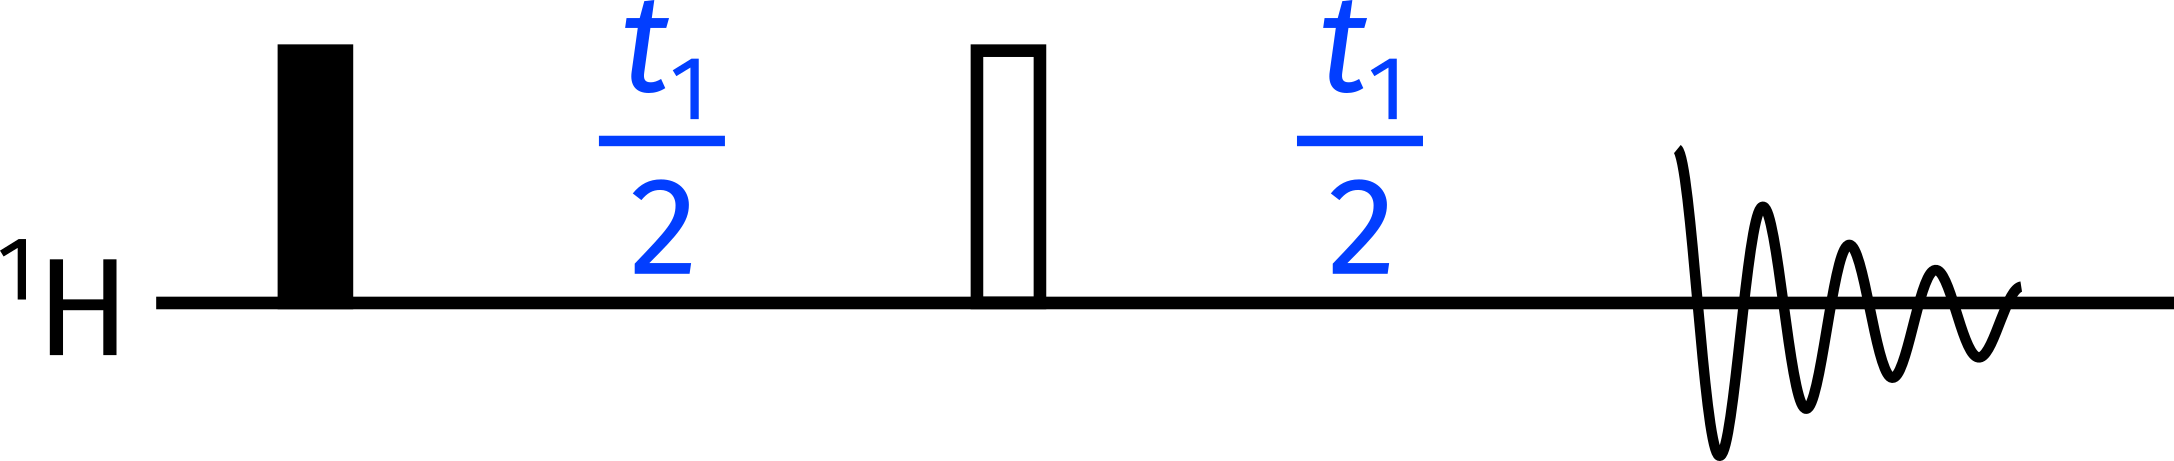
\includegraphics[]{pp/jres.png}%
    \caption[2DJ pulse sequence]{Pulse sequence for the J-resolved (2DJ) experiment.}
    \label{fig:pp_jres}
\end{figure}

Before moving on to the discussion of how PSEs are implemented in practice, I insert a slight digression about \textit{J-resolved} (or \textit{2DJ}) \textit{spectroscopy}, which is very closely related to pure shift NMR.
The basic 2DJ sequence involves a spin echo of duration $t_1$, immediately followed by detection (\cref{fig:pp_jres}).
If we only consider a single operator and reuse the analysis above, setting the spin echo delay $\tau$ to be $t_1/2$ instead, then we have that
\begin{equation}
    \label{eq:2dj_operator_analysis}
    I_{1+}I_{2\alpha} \xrightarrow[]{t_1/2} \xrightarrow[]{180^\circ} \xrightarrow[]{t_1/2} \exp(-\mi \pi J t_1) I_{1-}I_{2\beta}.
\end{equation}
This yields a complex signal of the form
\begin{equation}
    \label{eq:2dj_signal}
    s(t_1, t_2) = \exp(-\mathrm{i}\pi J t_1) \exp[\mi(\Omega_1 - \pi J) t_2],
\end{equation}
which when Fourier transformed yields a phase twist lineshape at $(-\pi J, \Omega_1 - \pi J)$.
The other component on spin 1 (starting from $I_{1+}I_{2\beta}$) likewise yields a phase twist at $(\pi J, \Omega_1 + \pi J)$.
It has long been known that \textit{shearing} this 2DJ spectrum by $45^\circ$ (i.e.\ moving each data point $(\Omega_1, \Omega_2)$ to $(\Omega_1, \Omega_2 - \Omega_1)$) generates a spectrum which only has chemical shift information in the $\omega_2$ dimension.
After magnitude-mode processing, projection of this spectrum onto the $\omega_2$ axis, for example, would in principle yield a pure shift spectrum.\footnote{Or equivalently, projection of the unsheared spectrum along a $45^\circ$ axis\autocite{Aue1976JCP}.}
This is true, but in practice the phase twist lineshapes cause the resulting resolution to be very poor, which defeats the purpose of using a pure shift spectrum.
To circumvent this issue, a number of special processing techniques have been proposed\autocite{Xu1991JMR,Nuzillard1996JMRSA,Simova1997JMR} (see also references therein); but more ideally, we want a phase-sensitive 2DJ spectrum, which can be obtained by recording a pair of `echo' and `antiecho' signals:%
\footnote{The terms `echo' and `antiecho' refer to the relative senses of the coherences evolving during $t_1$ and $t_2$: in the echo spectrum these have opposite signs, e.g.\ $I_zS_+$ and $I_-$ in the HSQC, and in the antiecho spectrum they have the same sign. As pointed out by Pell and Keeler\autocite{Pell2007JMR}, this is not really appropriate for the 2DJ experiment since each half of $t_1$ has a coherence with a different sense, but we will stick to this nomenclature as the underlying concept is very similar to that of echo--antiecho processing.}
\begin{align}
    s_\text{echo}(t_1, t_2) &= \exp(\mathrm{i}\pi J t_1) \exp[\mi(\Omega_1 - \pi J) t_2] \label{eq:2dj_signal_echo} \\
    s_\text{antiecho}(t_1, t_2) &= \exp(-\mathrm{i}\pi J t_1) \exp[\mi(\Omega_1 - \pi J) t_2] \label{eq:2dj_signal_antiecho}
\end{align}
These can be processed in the same way as described in \cref{subsec:theory__2dnmr} to yield double absorption-mode lineshapes.
The antiecho signal (\cref{eq:2dj_signal_antiecho}) is of course the same as in \cref{eq:2dj_signal}, but to obtain the echo signal in \cref{eq:2dj_signal_echo}, we require a different pulse sequence with a PSE inserted just prior to detection:
\begin{align}
    \label{eq:2dj_signal_echo_ctp}
    I_{1-}I_{2\alpha} \xrightarrow[]{t_1/2} &\exp[\mi(\Omega_1 + \pi J)t_1/2] I_{1-}I_{2\alpha} \\
    \xrightarrow[]{180^\circ} &\exp[\mi(\Omega_1 + \pi J)t_1/2] I_{1+}I_{2\beta} \\
    \xrightarrow[]{t_1/2} &\exp(\mi \pi J t_1) I_{1+}I_{2\beta} \\
    \xrightarrow[]{\text{PSE}} &\,c \exp(\mi \pi J t_1) I_{1-}I_{2\beta} \\
    \xrightarrow[]{t_2} &\,c \exp(\mi \pi J t_1) \exp[\mi(\Omega_1 - \pi J) t_2].
\end{align}
(Note that we began the analysis with a different operator here, $I_{1-}I_{2\alpha}$, in order to end up with the same $I_{1-}I_{2\beta}$ operator just before detection.)
In order to apply echo--antiecho processing, the decrease in sensitivity by a factor of $c$ must also be applied to the antiecho spectrum: this can be done by simply inserting the PSE immediately after the initial excitation pulse, which simply scales all operators down by $c$.
Thus, we see that \textit{exactly the same PSE} allows us to generate pure shift spectra as well as absorption-mode 2DJ spectra: this has been previously demonstrated using various PSEs.\autocite{Pell2007JMR,Foroozandeh2015CC}

In fact, the same formalism can be used to describe a family of small flip angle COSY experiments, including ECOSY\autocite{Griesinger1985JACS,Sorensen1985JACS,Griesinger1986JCP} and $z$-COSY\autocite{Oschkinat1986JMR,Pell2007MRC,Moutzouri2020ACIE}; these are also closely related to pure shift NMR.
In particular, the anti $z$-COSY experiment is a precursor to PSYCHE, and is analysed in \cref{subsec:pureshift__psyche_analysis}.
However, a full discussion of these is beyond the scope of this thesis.
